\label{ch:unlock_mechanism}
Πριν να εξηγήσουμε τον τρόπο κατασκευής και λειτουργίας του PiLock, είναι αναγκαίο να αναφερθούμε στον τρόπο λειτουργίας των περισσότερων κλειδαριών σπιτιών, πολυκατοικιών ή και γραφείων.

Το σύστημα ξεκλειδώματος που χρησιμοποιείται στις περισσότερες κατοικίες αποτελείται από 2 εντελός ξεχωριστά και ανεξάρτητα συστήματα: Το σύστημα του θυροτηλεφώνου, δηλαδή το σύστημα μέσω του οποίου γίνεται η αναγνώριση του επισκέπτη (μέσω φωνής ή/και εικόνας), και το σύστημα ενεργοποίησης της κλειδαριάς. Στην παρούσα διατριβή θα αναφερθούμε αποκλειστικά στο δεύτερο σύστημα.

Οι ηλεκτρικές κλειδαριές που χρησιμοποιούνται σε πολυκατοικίες συνήθως αποτελούνται από ένα μάνταλο το οποίο, όταν το σύστημα ενεργοποιηθεί μέσω ρεύματος, απελευθερώνεται με αποτέλεσμα να μπορεί ελεύθερα η πόρτα να ανοίξει.

\begin{figure}[h]
	\centering
		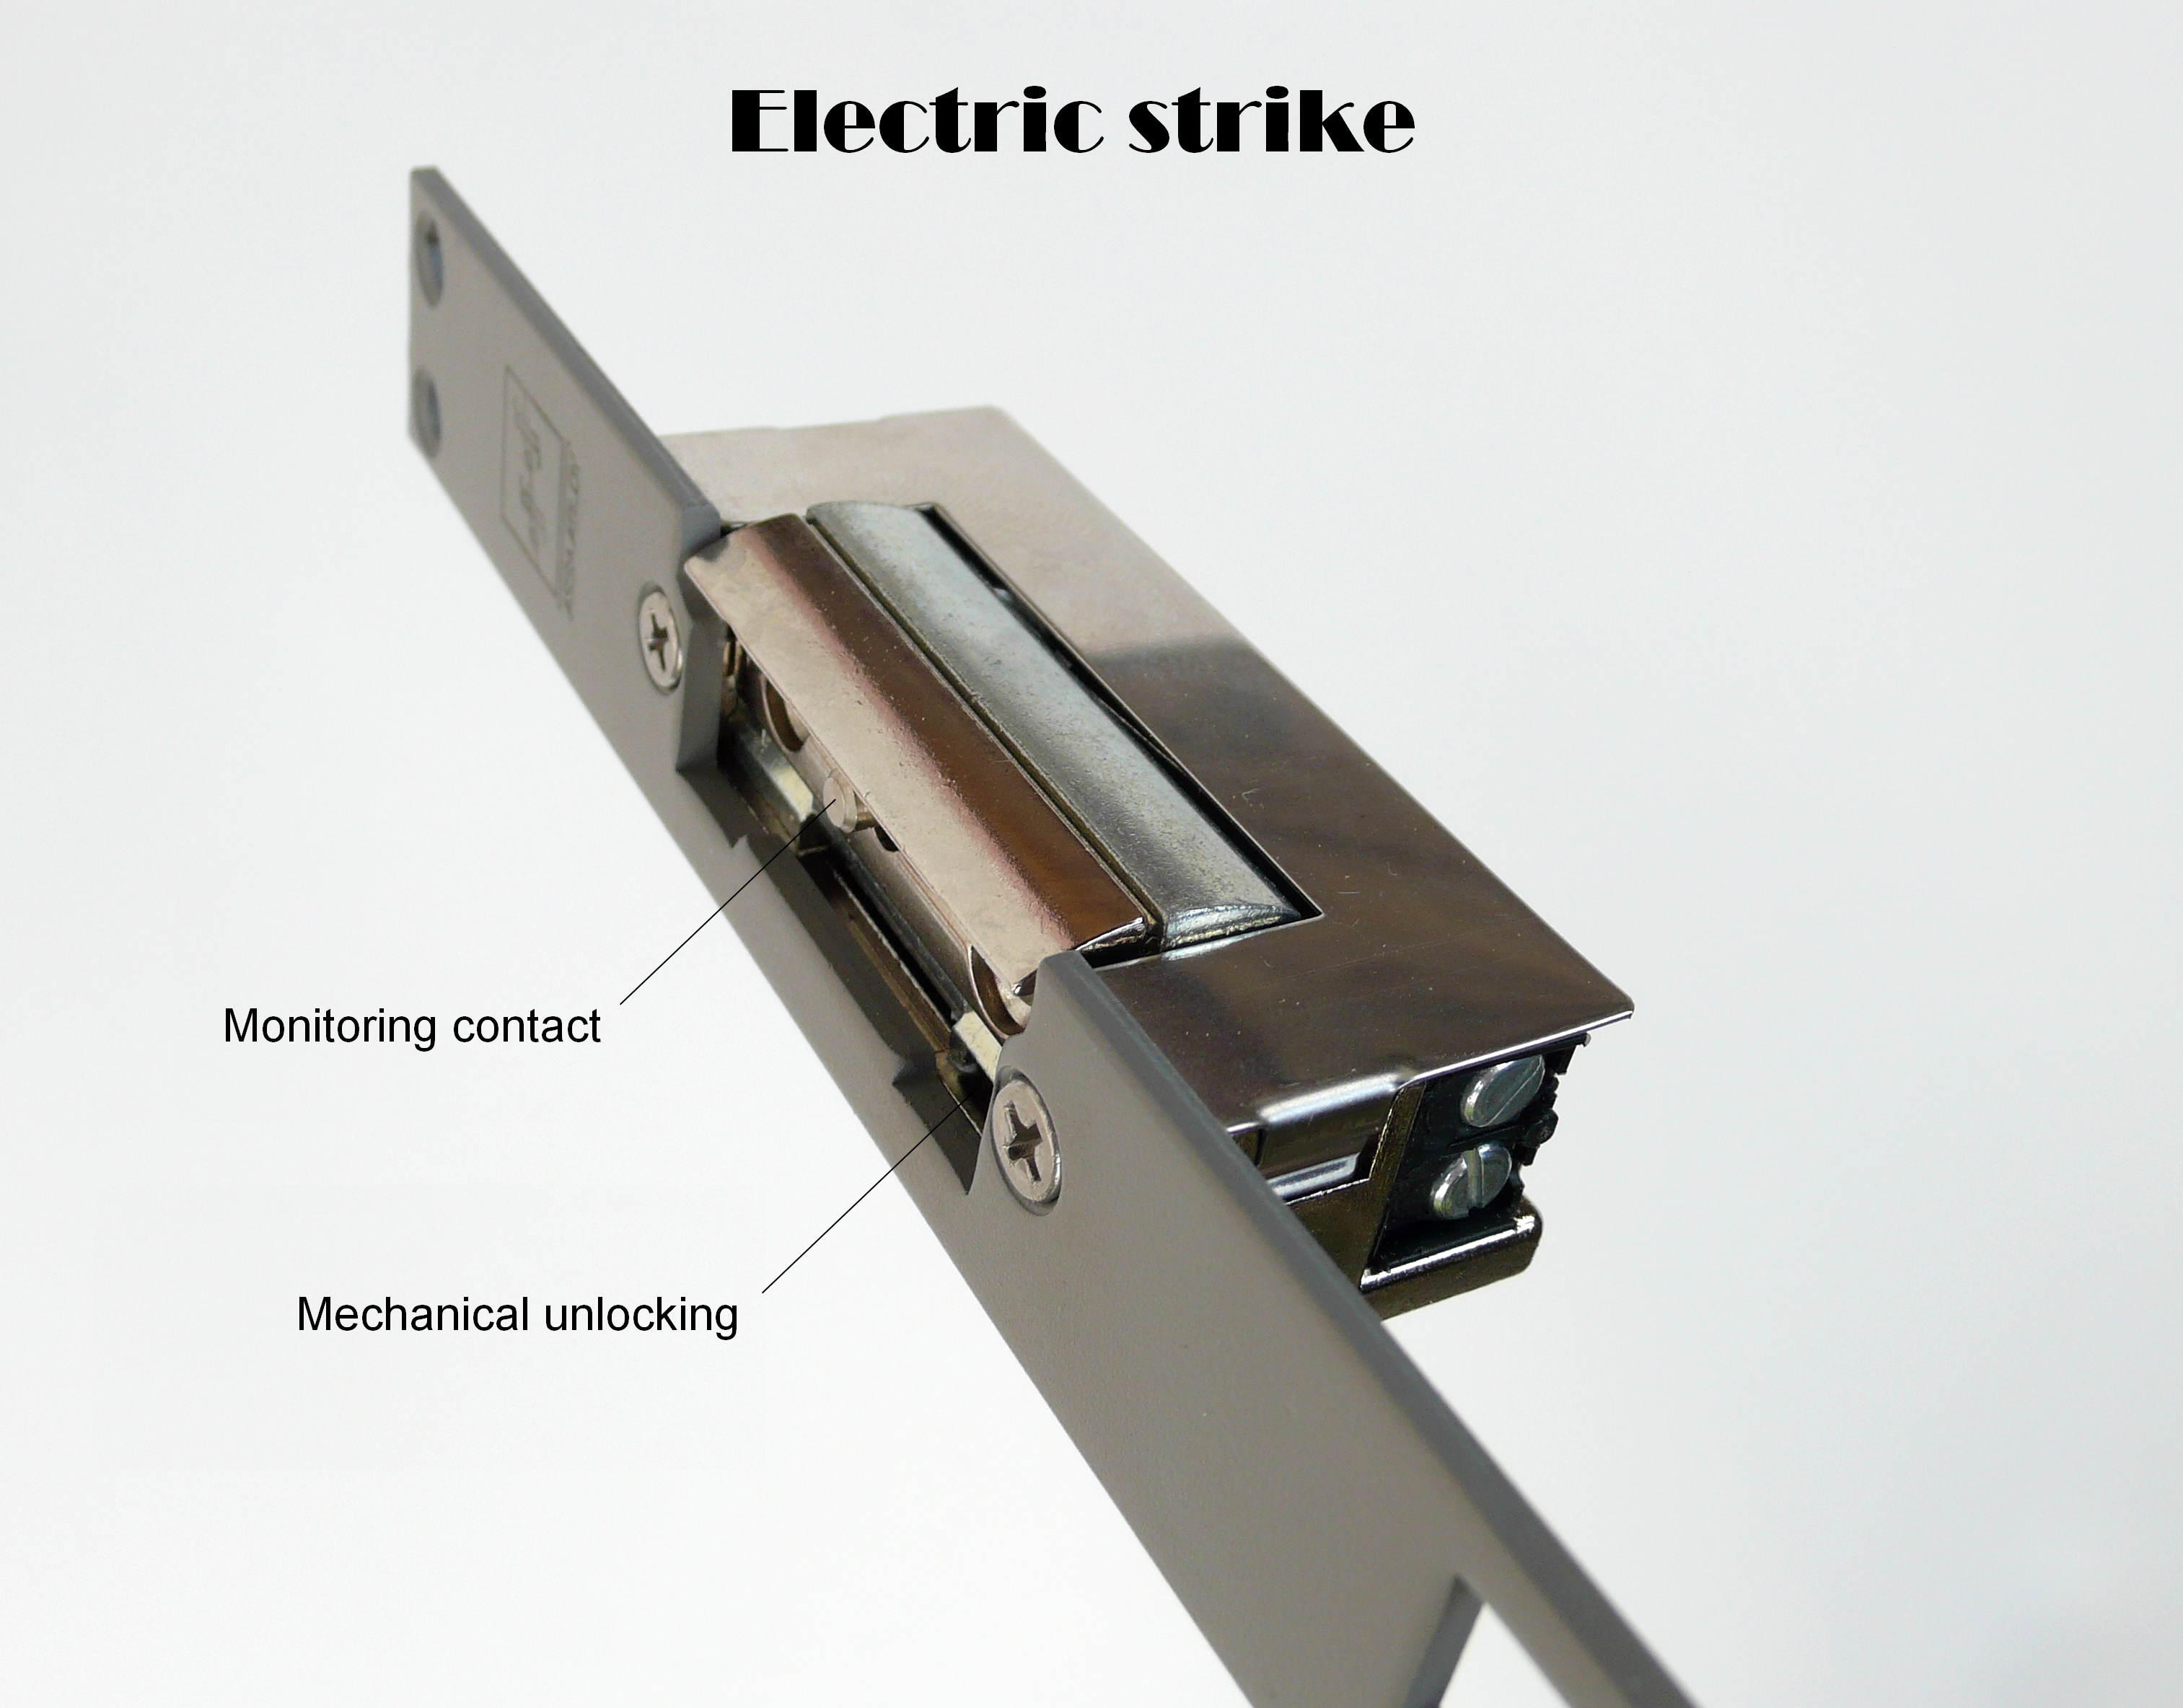
\includegraphics[width=0.5\textwidth,height=0.5\textheight,keepaspectratio]{Electric_strike.jpg}
	\caption{Ηλεκτρική κλειδαριά πολυκατοικίας με σύστημα καταγραφής κατάστασης κλειδώματος}
\end{figure}

Η ενεργοποίηση του παραπάνω συστήματος γίνεται μέσω ενός διακόπτη αναρτημένου πάνω στο θυροτηλέφωνο του κάθε διαμερίσματος. Η τροφοδοσία των συστημάτων αυτών μπορεί να γίνεται είτε μέσω απευθείας τροφοδοσίας από το ηλεκτρικό δίκτυο, είτε μέσω κάποιου μετασχηματιστή σε χαμηλότερες τάσεις.

Προκεικένου να μπορέσουμε να ελέγξουμε το σύστημα ξεκλειδώματος, θα πρέπει να μπορέσουμε να βάλουμε έναν δεύτερο διακόπτη, να λειτουργεί παράλληλα με τον πρώτο.  %TODO Refer to next chapter.

Για να γίνει αυτό, θα πρέπει να εντοπιστεί το κύκλωμα που συνδέεται με τον ήδη υπάρχοντα διακόπτη ξεκλειδώματος (του θυροτηλεφώνου) και να τοποθετηθούν 2 καλώδια σε παράλληλη σύνδεση με τον ήδη υπάρχοντα διακόπτη.

Για τον εντοπισμό θα πρέπει να αποσυνδεθεί ο διακόπτης από τον τοίχο, λύνοντας τις βίδες οι οποίες τον συγκρατούν. Προκειμένου να γίνει υπο ασφαλές συνθήκες, συνίσταται να απενεργοποιηθεί η παροχή ρεύματος στο παρόν τμήμα της οικίας, μέχρι να ολοκληρωθεί η εγκατάσταση. Αυτό μπορεί να γίνει είτε κατεβάζοντας την ασφάλεια που αντοιστοιχεί στο συγκεκριμένο τμήμα της κατοικίας, από τον ηλεκτρικό πίνακα, είτε απενεργοποιόντας τον γενικό διακόπτη τροφοδοσίας της κατοικίας.

Η τελική εγκατάσταση θα υπογραμμιστεί σε επόμενο κεφάλαιο.